\chapter{Metodi di anomaly detection}
\label{chap:methods}

\section{Modelli di apprendimento}
I modelli di apprendimento sono algoritmi che utilizzano dati per apprendere come effettuare una determinata attività come la classificazione o la regressione. Ci sono diverse categorie di modelli di apprendimento, tra cui:
\begin{enumerate}
\item \textbf{Modelli supervisionati}: utilizzano dati etichettati (in cui la risposta corretta è nota) per apprendere in base alla loro etichetta.
\item \textbf{Modelli non supervisionati}: utilizzano dati non etichettati (in cui la risposta corretta non è nota) per scoprire relazioni e strutture all'interno dei dati.
\end{enumerate}

I modelli di apprendimento sono utilizzati in molte aree, tra cui il riconoscimento delle immagini, il processamento del linguaggio naturale, la previsione delle serie temporali, la robotica e molte altre.

\subsection{Modelli supervisionati}
I modelli di apprendimento supervisionato sono una categoria di algoritmi di apprendimento automatico che utilizzano dati etichettati per "imparare" come effettuare una determinata attività. Il processo di apprendimento consiste nell'allenare il modello su un insieme di dati di addestramento etichettati, in cui la risposta corretta è nota, e quindi testarlo su un insieme di dati di test per valutare le sue prestazioni. Quando il modello riceve un nuovo dato da predire lo compara rispetto ciò che ha appreso durante la fase di allenamento. I principali task dei modelli supervisionati sono due: classificazione e regressione.

\subsubsection{Classificazione}
La classificazione è il problema di identificare a quale categoria o classe un'osservazione appartiene. Un classificatore, definito come \(\hat{c}\), è una funzione che mappa uno spazio di input \(X\), che definisce come i dati sono descritti, ad uno spazio di output \(C=\{C_1,...,C_k\}\) ovvero il set finito di etichette
\[\hat{c}: X \rightarrow C\]
Nel campo dell'apprendimento supervisionato gli esempi sono accompagnati da delle etichette e sono dunque definiti come \((x,c(x))\in X\times C\) dove \(x \in X\) e \(c(x)\) è la corretta classe di \(x\). Il task di classificazione è quello di andare a costruire la funzione \(\hat{c}\) che meglio approssima la funzione reale \(c\) non solo nei dati di training ma nell'intero spazio \(X\). Questa è una condizione importante perché vogliamo che il classificatore generalizzi bene e non faccia over-fitting. Over-fitting si ha quando un classificatore ha performance molto alte sui dati di training ma molto basse sui dati di test.
Esistono 4 tipi di classificatori:
\begin{enumerate}
\item \textbf{Classificatori binari}: è il più semplice in quanto l'insieme delle classi contiene solo due elementi: \(C=\{C_1,C_2\}\).
\item \textbf{Classificatori a score}: sono delle funzioni che assegnano uno score alla predizione: \(\hat{s} = X\rightarrow R^k\) dove \(X\) rappresenta lo spazio di input mentre l'output è definito da un vettore di \(k\) numeri reali: 
\[(\hat{s}_1 (x),...,\hat{s}_k(x))\]
In questo vettore, il componente k-esimo è lo score assegnato alla classe \(C_k\) per l'istanza \(x\). Generalizzando, per ogni istanza \(x\) esiste un vettore \(\hat{s}(x)\) contenente i punteggi \(\hat{s}_k(x)\) per ogni classe \(k\) di \(C\).
\item \textbf{Classificatori probabilistici}: eredita delle caratteristiche dai classificatori a score con la differenza che il valore di ogni componente del vettore di output di una istanza \(x\) rappresenta la probabilità che quell'istanza ricada nella classe \(k\). Essendo probabilità, la somma totale di tutti i valori all'interno del vettore corrisponde a 1.
\item \textbf{Classificatori multiclasse}: sono un'estensione dei classificatori binari con un insieme delle classi maggiore di due elementi: \(C=\{C_1,...,C_k\}\). 
\end{enumerate}

\subsubsection{Regressione}
All'interno del task di regressione siamo di fronte non più ad un codominio finito, come nel caso della classificazione, ma un codominio rappresentato dall'insieme dei numeri reali \(R\). I modelli di regressione sono quindi definiti da una funzione
\[\hat{f}: X \rightarrow \mathbb{R}\]
Il problema di apprendimento è anche qui quello di trovare la funzione \(\hat{f}\) che meglio approssima la funzione reale \(f: (x_i, f(x_i))\) per ogni \(x\in X\).
Cambiando l'obiettivo della funzione da un numero relativamente piccolo di classi a uno spazio di soluzioni infinito, l'algoritmo cercherà di stimare i valori associati a ciascun esempio nel modo più accurato possibile, il che porterà al problema dell'overfitting. Tenendo presente che è necessario accettare un equilibrio tra accuratezza e approssimazione delle soluzioni, è inevitabile, di fronte alle normali oscillazioni dei dati, che il modello non possa catturarle con precisione. Il vero scopo di un modello di regressione è quello di approssimare l'andamento della funzione $f$ nel miglior modo possibile. La Figura \ref{overfitting} mostra un esempio di problema di regressione: la linea rossa rappresenta una funzione che fa overfitting, ovvero è precisa sui dati di training. Questo comporta un basso livello di bias ma alta varianza: i dati nuovi non riuscirà a predirli con precisione. Le linee blu invece rappresentano modelli più "semplici" che generalizzano meglio, hanno quindi un bias più alto ed una varianza più bassa.

\begin{figure}[t]
	\centering
	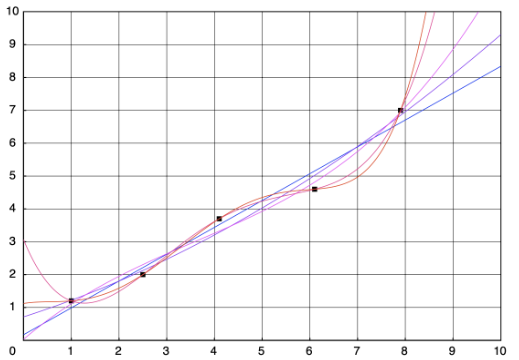
\includegraphics[width=10cm, scale=1]{images/overfitting}
	\caption{Overfitting}
	\label{overfitting}
\end{figure}


\subsection{Modelli non supervisionati}
L'apprendimento non supervisionato è una categoria di algoritmi di apprendimento automatico che utilizzano dati non etichettati per "imparare" da essi. In contrasto con l'apprendimento supervisionato, dove ci sono dati etichettati con le risposte corrette, l'apprendimento non supervisionato non ha accesso alle risposte corrette, ma cerca di scoprire relazioni o strutture all'interno dei dati.

Ci sono diverse tipologie di algoritmi di apprendimento non supervisionato, tra cui:
\begin{itemize}
\item \textit{Clustering}: utilizzato per raggruppare gli esempi in base alle loro similitudini.
\item \textit{Riduzione della dimensionalità}: utilizzato per ridurre la dimensionalità dei dati.
\item \textit{Analisi di componenti principali (PCA)}: utilizzato per individuare le componenti principali dei dati.
\item \textit{Anomaly Detection}: utilizzato per identificare dati anomali o fuori dalla norma.
\item \textit{Modelli Generativi}: utilizzati per generare nuovi dati.


\end{itemize}
Nel rilevamento supervisionato delle anomalie, se vogliamo che un modello sia in grado di rilevare le anomalie, bisogna allenare il sistema in modo molto preciso sia nell'identificare il comportamento normale che quello anomalo.
Tuttavia, i comportamenti normali possono essere molteplici così come i
comportamenti in presenza di anomalie e questo porta con se la necessità di fornire una grande quantità di dati etichettati per catturare più comportamenti possibili. Purtroppo non è sempre possibile in quanto le anomalie sono eventi rari e se il dataset di addestramento è relativamente piccolo, anche il numero di anomalie non sarà sufficientemente grande, rendendo difficile la loro classificazione. 
Pertanto, l'apprendimento non supervisionato si adatta perfettamente al problema del rilevamento delle anomalie, poiché non è necessario etichettare i dati. Inoltre, una parte delle anomalie derivano da nuovi comportamenti del sistema e per definizione questi comportamenti non possono essere classificati correttamente con i metodi di rilevamento delle anomalie supervisionati senza effettuare prima un re-training.


\section{Valutazione del modello}
La valutazione del modello è necessaria per quantificarne le prestazioni. La
scelta delle metriche e delle tecniche di valutazione dipende dal task di apprendimento come la classificazione o la regressione. 
In questa sezione ci si concentrerà sulle tecniche e sulle metriche più famose utilizzate per valutare la performance di un modello su un determinato compito.

\subsubsection{Tecniche}
\begin{itemize}
	\item \textbf{Random Split} genera in maniera casuale i tre insiemi di train, test e validazione. Il vantaggio di questo metodo è che c'è una buona probabilità che la popolazione originale sia ben rappresentata in tutti e tre gli insiemi, impedendo quindi un campionamento distorto dei dati.
	\item \textbf{Time Based Split} viene applicato sulle serie temporali in cui non è possibile effettuare una suddivisione casuale dei dati in quanto si andrebbe a perdere informazioni come trend o stagionalità. 
	      In questi casi, si utilizza una suddivisione temporale in cui, ad esempio, l'insieme di train può contenere i dati più vecchi, mentre quelli più recenti sono assegnati all'insieme di test. Per evitare l'overfitting introdotto da questo metodo, una variante a finestre di scorrimento è preferibile: il modello viene allenato iterativamente più volte su una finestra temporale e valutato sulla parte restante dei dati, per poi allargare la finestra di training ad ogni iterazione (riducendo così quella di valutazione).
	\item \textbf{K-Fold Cross Validation} tiene in considerazione due tipologie di dati: il test set ed il train set. Per formare questi insiemi, genera in modo casuale $k$ gruppi di dati ed iterativamente vengono usati $k-1$ gruppi per il training ed un gruppo per il test.
	\item \textbf{Stratified K-Fold} è simile al Cross Validation ma con la differenza che questo metodo tiene in considerazione la distribuzione delle classi dei dati, generando quindi gruppi con rateo simile al dataset originale.
\end{itemize}


\subsubsection{Metriche}
Alla base di tutte le metriche di valutazione vi è la tabella di contingenza. Questa tabella permette di valutare le performance di un modello andando a relazionare, in più modi, le predizioni di un modello con le etichette reali.

La Tabella \ref{contigency-table} mostra la struttura della tabella di contingenza.  La prima colonna contiene il numero delle predizioni positive fatte da un modello divise se queste sono effettivamente positive o negative. La seconda colonna funziona allo stesso modo ma per le predizioni negative. La terza colonna invece rappresenta la somma dei punti che sono realmente positivi e realmente negativi.
Riassumendo:
\begin{itemize}
\item \textit{True Positive}: punti realmente positivi che sono predetti come tali.
\item \textit{False Positive}: punti realmente positivi ma predetti come negativi.
\item \textit{False Negative}: punti realmente negativi ma predetti come positivi.
\item \textit{True Negative}: punti realmente negativi che sono predetti come tali.
\item \textit{Pos}: Somma totale dei punti realmente positivi.
\item \textit{Neg}: Somma totale dei punti realmente negativi.
\end{itemize}

\begin{table}[]
\centering
	\caption{\label{contigency-table}Tabella di contingenza}

\begin{tabular}{|l|l|l|l|}
\hline
                 & \textbf{Predizioni +} & \textbf{Predizioni -} & \textbf{Totale} \\ \hline
\textbf{Reale +} & TP                    & FN                    & Positivi        \\ \hline
\textbf{Reale -} & FP                    & TN                    & Negativi        \\ \hline
\end{tabular}
\end{table}

Definiamo prima $T_e$ come l'insieme dei punti del nostro dataset, a questo punto è possibile introdurre tutte le misure di performance:
\begin{itemize}
\item \textit{Accuracy}: è il rapporto tra i punti correttamente classificati rispetto al totale dei punti.
\[\frac{1}{|T_e|} \sum_{x \in T_e} I[\hat{c}(x)=c(x)]\]
\item \textit{Error Rate}: è il rapporto tra i punti erroneamente classificati rispetto al totale dei punti, in breve \(1-accuracy\).
\[\frac{1}{|T_e|} \sum_{x \in T_e} I[\hat{c}(x)\neq c(x)]\]
\item \textit{True Negative Rate / Specificity}: è il rapporto tra i punti classificati correttamente come negativi rispetto al numero totale di punti realmente negativi.
\[\frac{\sum_{x \in T_e} I[\hat{c}(x)=c(x)=-]}{\sum_{x \in T_e} I[c(x)=-]}\]
\item \textit{True Positive Rate / Recall}: è il rapporto tra i punti classificati correttamente come positivi rispetto al numero totale di punti realmente positivi.
\[\frac{\sum_{x \in T_e} I[\hat{c}(x)=c(x)=+]}{\sum_{x \in T_e} I[c(x)=+]}\]
\item \textit{Precision}: è il rapporto tra i punti correttamente classificati come positivi rispetto al numero di punti classificati come positivi.
\[\frac{\sum_{x \in T_e} I[\hat{c}(x)=c(x)=+]}{\sum_{x \in T_e} I[\hat{c}(x)=+]}\]
\item \textit{F-Measure Score}: è la media armonica tra precision e recall.
\[F_\beta=\frac{\left(1+\beta^2\right) \cdot(\text { precision } \cdot \text { recall })}{\left(\beta^2 \cdot \text { precision }+\text { recall }\right)}\]
\end{itemize}
Quest'ultima misura introduce il parametro $\beta$ che serve per dare più o meno peso alle componenti della formula: se $\beta = 1$, allora sia la precision che la recall avranno lo stesso peso, un valore di $\beta < 1$ da più peso alla precision, infine un valore di $\beta > 1$ da più peso alla recall.

In generale non esiste una misura migliore e bisogna fare un'attenta valutazione su quale sia la preferibile rispetto al task da risolvere.
Ad esempio bisogna tenere in considerazione se c'è una prevalenza di punti di una classe. Accuracy è preferibile quando ci si aspetta una distribuzione equa delle classi. Quando i falsi-negativi non sono di interesse, ma lo sono i falsi-positivi, precision è preferibile; al contrario quando i falsi-negativi sono molto importanti e non ci interessa dei falsi-positivi, recall è la scelta corretta.
F-Measure invece è necessaria quando si cerca un bilanciamento tra precision e recall dando importanza a entrambi i falsi-positivi ed i falsi-negativi. 
All'interno del contesto SKF e Anomaly Detection le anomalie sono sicuramente importanti da riconoscere e marcarle come negative, quindi falsi-negativi, potrebbe risultare in problemi alla linea di produzione. Ma allo stesso tempo un modello che produce molti più positivi di quanto deve risulterebbe in una perdita di fiducia da parte dell'operatore che inizierebbe semplicemente ad ignorare il feedback del modello. Per questo motivo la scelta della metrica di valutazione è ricaduta sulla F-Measure.



\section{Modelli di apprendimento automatico}
In questa sezione vengono proposti diversi algoritmi e metodi di apprendimento automatico per l'Anomaly Detection, raggruppati per categoria.
I seguenti algoritmi sono implementati all'interno della libreria pubblica PyOD\footnote{Python Outlier Detection (PyOD): https://github.com/
yzhao062/pyod} e TODS\footnote{Automated Time-series Outlier Detection System
 (TODS): https://github.com/datamllab/tods} ed utilizzati nel processo di Model Selection discusso nei capitoli successivi.

\subsection{Modelli lineari}
I modelli lineari sono un tipo di algoritmo di Machine Learning utilizzato per fare previsioni. Essi rappresentano la relazione tra le variabili indipendenti (chiamate anche feature) e la variabile dipendente (chiamata anche obiettivo) con una equazione lineare. La forma generale di un modello lineare è: 
\[ Y = B_0 + B_1X_1 + B_2X_2 + ... + B_n \cdot X_n\]
dove $ Y $ è la variabile dipendente,  \(X_1, X_2, ..., X_n\)  sono le variabili indipendenti mentre \( B_0, B_1, B_2, ..., B_n\) sono i coefficienti del modello che vengono "appresi" dai dati.

\subsubsection{PCA}
La PCA \cite{shyu2003novel} è una riduzione lineare della dimensionalità che utilizza la Singular Value Decomposition dei dati per proiettarli in uno spazio dimensionale inferiore. Si tratta di spiegare la struttura di varianza-covarianza di una serie di variabili attraverso alcune nuove variabili che sono funzioni di quelle originali. Le componenti principali sono particolari combinazioni lineari delle \textit{p} variabili casuali  \(X_1, X_2, ..., X_p\) con tre importanti proprietà: (1) le componenti principali non sono correlate, (2) la prima componente principale ha la varianza più elevata, la seconda componente principale ha la seconda varianza più elevata e così via, e (3) la variazione totale in tutte le componenti principali combinate è uguale alla variazione totale delle variabili originali \(X_1, X_2, ..., X_p\). 
Queste componenti principali sono ricavabili da un'analisi degli autovalori della matrice di covarianza o della matrice di correlazione di \(X_1, X_2, ..., X_p\).
In questa procedura, la matrice di covarianza dei dati può essere decomposta in vettori ortogonali, detti autovettori, associati ad autovalori. Gli autovettori con alti autovalori catturano la maggior parte della varianza dei dati. Pertanto, un iperpiano a bassa dimensionalità costruito da \textit{k} autovettori può catturare la maggior parte della varianza dei dati. Tuttavia, gli outlier sono diversi dai punti di dati normali, cosa che è più evidente sull'iperpiano costruito dagli autovettori con autovalori piccoli.
Di conseguenza, i punteggi degli outlier possono essere ottenuti come la somma della distanza proiettata di un campione su tutti gli autovalori.

\subsubsection{K-PCA}
Kernel-PCA \cite{hoffmann2007kernel} è un'estensione non lineare di PCA. I dati di input sono mappati in uno spazio infinitesimale da cui K-PCA estrae le componenti principali. I tipi di kernel usati possono essere: lineare, polinomiale, sigmoidale o radiale.



\subsubsection{Auto-Regressivo}
In un modello a regressione multipla viene fatta previsione di una variabile di interesse attraverso una combinazione lineare di predittori. Un modello Auto Regressivo, invece, fa previsione di questa variabile di interesse usando una combinazione lineare su \textit{valori passati} di questa variabile. Il termine auto-regressione indica una regressione della variabile fatta su se stessa.
Di conseguenza, un modello auto-regressivo di ordine \textit{p} può essere scritto come:
\[y_t=c+\phi_1 y_{t-1}+\phi_2 y_{t-2}+\cdots+\phi_p y_{t-p}+\varepsilon_t\]
dove $\varepsilon_t$ è rumore bianco. Può essere visto come una regressione multipla ma con valori ritardati di $y_t$ come predittori. 
La deviazione di un valore predetto rispetto a quello reale viene usato come outlier score.

\subsubsection{MCD}
Minimum Covariance Determinant (MCD) \cite{rousseeuw1999fast, hardin2004outlier} è un metodo per stimare la media e la matrice di covarianza andando a minimizzare l'influenza delle anomalie. L'idea alla base è quella di stimare questi valori andando a selezionare un sottoinsieme dei dati nella quale le anomalie o sono completamente assenti o sono il meno possibile.
Immaginando un approccio brute-force, l'algoritmo itera su ogni possibile sottoinsieme dei dati di una dimensione specifica. Vengono poi stimati la media e la matrice di covarianza per ogni sottoinsieme e poi vengono mantenuti soltanto i valori per il sottoinsieme che ha il determinante della matrice di covarianza più piccolo. Il motivo di questo è perché il determinante di una matrice di covarianza indica quanto è larga una distribuzione. Di conseguenza MCD cerca di minimizzare questo andando a prendere la distribuzione più compatta. Questo consente di escludere le anomalie che saranno situate lontane dal resto dei dati.

\subsubsection{LMDD}
Linear Method for Deviation-based Outlier Detection (LMDD) \cite{arning1996linear} impiega il concetto di Smoothing Factor il quale indica quanto può essere ridotta la misura di dissimilarità andando a rimuovere un sottoinsieme degli elementi dal dataset. La funzione di dissimilarità può essere qualsiasi misura di dispersione come la varianza, inter-quantile range, mediana ecc.
I punti rimossi che riducono maggiormente questa misura di dissimilarità possono essere valutati come anomalie.

\subsection{Modelli non lineari}
I modelli non lineari riescono a modellare relazioni non lineari nei dati, catturando relazioni più complesse e anche non linearmente separabili, limite dei modelli lineari.

\subsubsection{OCSVM}
Il metodo One Class Support Vector Machine (OCSVM) \cite{scholkopf2001estimating} è una versione derivata dalle Support Vector Machine al rilevamento di una sola classe. L'idea alla base consiste nel minimizzare l'ipersfera contenente i punti di una singola classe e considerare tutti i punti esterni alla sfera come outliers.
La Figura \ref{ocsvm} mostra un esempio del funzionamento di OCSVM.
\begin{figure}[t]
	\centering
	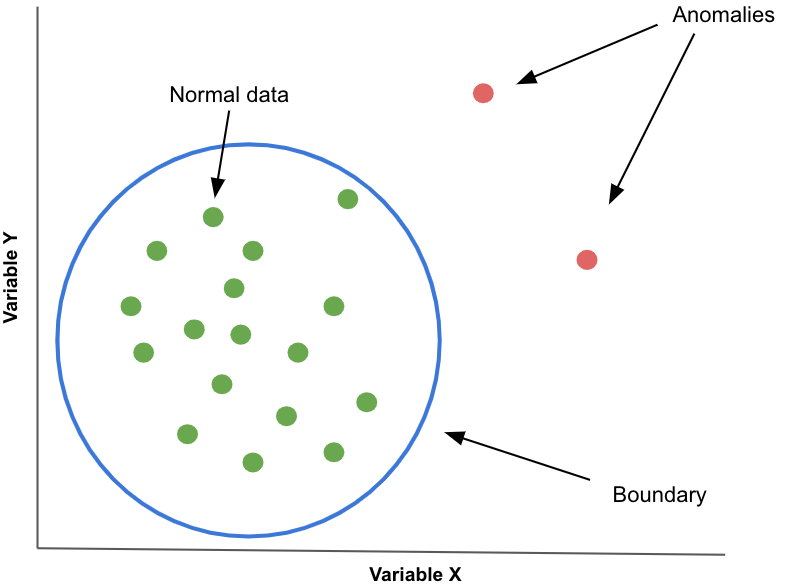
\includegraphics[width=8cm, scale=1]{images/ocsvm}
	\caption{OCSVM}
	\label{ocsvm}
\end{figure}

\subsection{Modelli a distanza}
I modelli non supervisionati basati sulla distanza sono una categoria di algoritmi che utilizzano la distanza tra i dati per scoprire relazioni e strutture nel dataset.

\subsubsection{KNN}
K-Nearest Neighbors (KNN) \cite{ramaswamy2000efficient,angiulli2002fast} è un algoritmo di apprendimento utilizzato per classificare oggetti in base alle loro proprietà. Dato un nuovo punto, l'algoritmo cerca i \textit{k} punti più simili (detti "vicini") tra quelli già classificati e assegna all'oggetto in esame la classe più comune tra i \textit{k} vicini trovati. La scelta del valore di \textit{k} è importante e può influire sulla sua accuratezza. In generale, un valore più alto di \textit{k} tende a ridurre la varianza del modello ma aumenta la sua bias.
Nel campo dell'Anomaly Detection non è di interesse assegnare la classe al punto in esame ma assegnare un punteggio di anomalia. Per un'osservazione, quindi, la sua distanza rispetto al \textit{k}-esimo punto più vicino rappresenta questo score.

\subsubsection{DBSCAN}
DBSCAN è un metodo di clustering che raggruppa i punti in aree ad alta densità e contrassegna i punti in regioni a bassa densità come anomali.
DBSCAN classifica quindi i punti in tre categorie. I punti centrali sono punti
contenenti almeno $minPts$ nel loro intorno definito da un parametro $\epsilon$. I border-point sono i punti che contengono almeno un punto centrale nel loro intorno, mentre gli altri punti sono considerati come rumore/anomalie. 


\subsubsection{LOF}
Local Outlier Factor (LOF) \cite{breunig2000lof} misura la deviazione locale di un dato punto rispetto ai suoi vicini. Sulla base del metodo dei KNN, la densità locale di questo punto viene valutata considerando la distanza rispetto ai suoi \textit{k} punti più vicini. Il punteggio di anomalia viene invece calcolato confrontando la sua densità locale con quella dei suoi \textit{k} vicini più prossimi. Un punteggio elevato indica una densità inferiore a quella dei suoi vicini e quindi potenzialmente un'anomalia. In Figura \ref{lof} è presente il funzionamento di LOF dove si possono notare cerchi più grandi per i punti più isolati.
\begin{figure}[t]
	\centering
	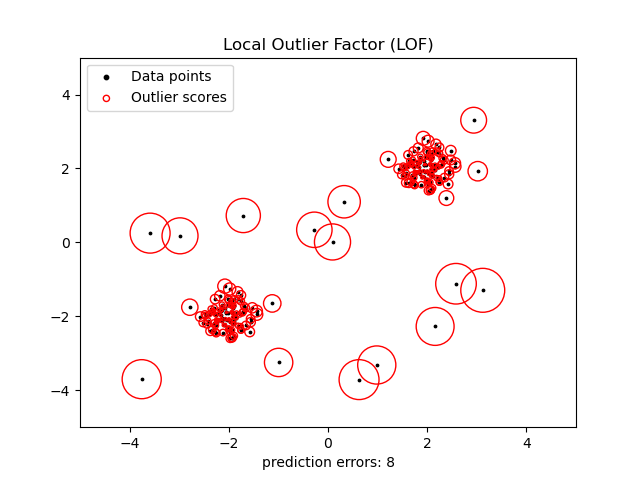
\includegraphics[width=10cm, scale=1]{images/lof}
	\caption{LOF}
	\label{lof}
\end{figure}

\subsubsection{COF}
Connectivity Outlier Factor (COF) \cite{tang2002enhancing} è un'evoluzione di LOF. Si basa sull'idea di assegnare un grado di anomalia ad ognuno dei punti, chiamato connectivity outlier factor.
Per ogni punto $x_i$, vengono selezionati i \textit{k} punti più vicini e viene generato il percorso minimo che attraversi tutti i \textit{k} punti partendo da $x_i$. Infine COF viene calcolato andando a fare una media delle distanze di ogni percorso di $x_i$ verso i suoi \textit{k} punti più vicini.

\subsubsection{CBLOF}
Cluster-Based Local Outlier Factor (CBLOF) \cite{he2003discovering} è anch'esso un evoluzione di LOF.
Come primo step, CBLOF riceve in input i dati ed un algoritmo di clustering per andare a formare dei cluster. Attraverso dei parametri va poi a definire quale cluster viene considerato "grande" e quale viene considerato "piccolo". Vengono poi calcolati gli outlier score per tutti i punti andando a considerare la dimensione del cluster a cui un punto appartiene e la distanza più vicina rispetto al centro di un cluster grande. Quindi più un cluster di appartenenza è piccolo e più il punto è lontano dal centro di un cluster grande, più lo score di anomalia sarà alto. 

\subsubsection{HBOS}
Histogram based outlier detection (HBOS) \cite{goldstein2012histogram} è un algoritmo di outlier detection che si basa sugli istogrammi assumendo indipendenza tra le features. Per ogni feature computa il rispettivo istogramma. Successivamente itera su ogni punto: se il valore di una feature di uno specifico punto $x_i$ rientra nella coda dell'istogramma, questo punto vede alzarsi lo score di anomalia. Questo passaggio viene ripetuto rispetto ad ogni feature e su tutti i punti.

\subsubsection{SOD}
Subspace outlier detection (SOD) \cite{kriegel2009outlier} cerca di trovare gli outlier andando a considerare diversi sottoinsiemi dello spazio multidimensionale delle feature. Per ogni osservazione, SOD esplora il sottoinsieme delle dimensioni che si dirama parallelamente dai punti vicini e determina quanto questa osservazione devia dai suoi vicini in questo sotto-spazio. 

\subsubsection{ROD}
Rotation-based Outlier Detection (ROD) \cite{almardeny2020novel},  è un algoritmo privo di parametri che non richiede conoscenza sulla distribuzione dei dati e funziona in modo intuitivo nello spazio tridimensionale, dove i vettori 3D, che rappresentano i punti, vengono ruotati attorno alla mediana geometrica due volte in senso antiorario utilizzando la formula di rotazione di Rodrigues. I risultati della rotazione sono parallelepipedi i cui volumi vengono analizzati matematicamente come funzioni di costo e utilizzati per calcolare le Deviazioni Assolute Mediane e ottenere così il punteggio di anomalia. Per dimensioni elevate > 3, il punteggio complessivo viene calcolato prendendo la media dei punteggi complessivi dei sottospazi 3D risultanti dalla scomposizione dello spazio dei dati originali.


\subsection{Modelli probabilistici}
I modelli probabilistici non supervisionati sono una categoria di algoritmi che utilizzano la probabilità per descrivere e generare i dati. Essi utilizzano una distribuzione di probabilità per rappresentare la relazione tra le variabili del dataset.
\subsubsection{KDE}
Kernel Density Estimation (KDE) \cite{latecki2007outlier} è l'applicazione di un "kernel smoothing" per la stima della probabilità. 
Siano $(x_1,...,x_n)$ osservazioni indipendenti e identicamente distribuite prese da una distribuzione univariata con una densità non conosciuta \textit{f} per qualsiasi punto \textit{x}. Siamo interessati nello stimare la forma di questa funzione \textit{f}. La funzione kernel di stima è:
\[\widehat{f}_h(x)=\frac{1}{n} \sum_{i=1}^n K_h\left(x-x_i\right)=\frac{1}{n h} \sum_{i=1}^n K\left(\frac{x-x_i}{h}\right)\]

Dove \textit{K} è il kernel, una funzione non negativa, e $h>0$ è un parametro di smoothing chiamato bandwidth. Un kernel con pedice $h$ è chiamato \textit{kernel scalato} ed è definito da: $Kh(x) = 1/h K(x/h)$. 
Il valore di $k$ deve essere scelto tenendo conto del trade-off bias/varianza.
I kernel più utilizzati sono: uniforme, triangolare e normale.
Le stime di densità con kernel sono fortemente correlate agli istogrammi, ma sono dotati di proprietà di smoothing o di valori continui usando appunto questi kernel.
La Figura \ref{kde_model} mostra un confronto tra un istogramma con una funzione di stima di densità con kernel.
L'applicazione di questo modello nell'Anomaly Detection avviene andando a generare, per un'osservazione, uno score di anomalia corrispondente al valore negativo del logaritmo della probabilità di densità.

\begin{figure}[t]
	\centering
	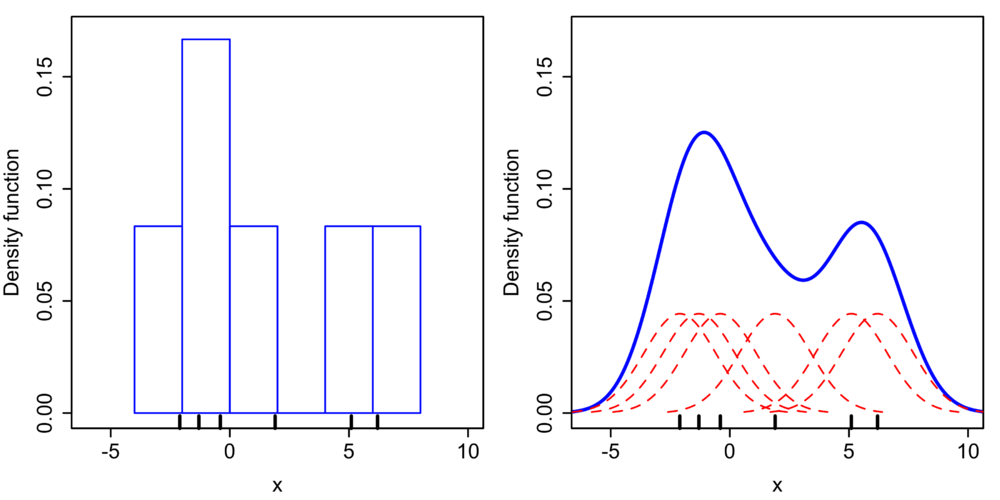
\includegraphics[width=10cm, scale=1]{images/kde_model}
	\caption{KDE}
	\label{kde_model}
\end{figure}


\subsubsection{GMM}
I GMM \cite{aggarwal2015outlier} sono una generalizzazione delle distribuzioni gaussiane e possono essere utilizzati per rappresentare qualsiasi serie di dati che possono essere raggruppati in più distribuzioni gaussiane. GMM è un modello probabilistico che presuppone che tutti i punti dati siano generati da una insieme di distribuzioni gaussiane con parametri sconosciuti e può essere utilizzato per il clustering, oppure per stimare la probabilità che un nuovo punto dati appartenga a ciascun cluster. Può essere inteso come un modello probabilistico in cui si ipotizzano distribuzioni gaussiane per ciascun gruppo, con medie e covarianze che ne definiscono i parametri.

Per la stima di questi parametri si esegue l'algoritmo di Expectation-Maximization chiamato così in quanto vengono alternate iterativamente due fasi: quella di expectation e quella di maximization. L'algoritmo parte inizializzando prima i parametri del GMM. A ogni iterazione, la fase di expectation calcola il valore atteso della funzione log-likelihood rispetto ai parametri correnti. Questa valore viene poi utilizzato per massimizzare la log-likelihood nella fase di massimizzazione.

È possibile adottare questo modello nell'Anomaly Detection allenandolo rispetto ad un set di dati e poi assegnando un punteggio ai nuovi punti: quelli significativamente diversi dal resto dei dati verranno marcati come anomalia.

\subsubsection{ABOD}
Angle Based Outlier Detection (ABOD) \cite{kriegel2008angle} si basa sull'idea di osservare l'angolo formato da un insieme di tre punti qualsiasi nello spazio delle feature multivariate. La varianza dell'ampiezza dell'apertura angolare risulta diversa per i punti anomali e per quelli normali: la varianza osservata è più alta per i punti inlier e più bassa per gli outlier, quindi tale misura può essere usata per separare punti normali da anomalie. ABOD funziona abbastanza bene nello spazio ad alta dimensionalità, a differenza di altre misure basate sulla distanza che soffrono della "curse of dimensionality" in quanto gli angoli possono fornire una rappresentazione migliore della vicinanza.
\begin{figure}[t]
	\centering
	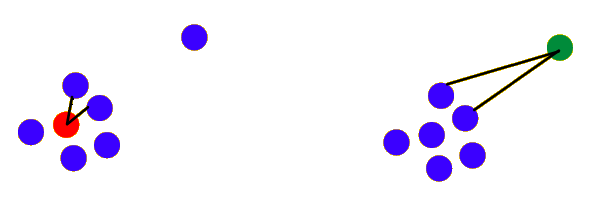
\includegraphics[width=10cm, scale=1]{images/abod}
	\caption{ABOD}
	\label{abod}
\end{figure}
Un esempio sull'idea alla base di ABOD è presente in Figura \ref{abod}.
Considerando il punto rosso come pivot, viene calcolato l'angolo racchiuso tra questo punto e qualsiasi altro punto dello spazio e con molta probabilità si noterà un'alta varianza tra questi valori. Questo andamento indica che il punto pivot fa parte di un cluster ad alta coesione.
Se si considera come pivot invece il punto verde e procedendo con gli stessi calcoli per ogni coppia di punti, la varianza angolare sarà molto più bassa, indice che quel punto è molto probabilmente un outlier.

\subsubsection{ECOD}
Empirical-Cumulative-distribution-based Outlier Detection (ECOD) \cite{li2021ecod} è un modello probabilistico che basa il suo funzionamento nel calcolare, per ogni punto $x_i \in X$, la probabilità che esista un punto almeno "estremo" come $x_i$.
ECOD prima stima la distribuzione dei dati di input senza l'ausilio di parametri esterni andando a computare la distribuzione cumulativa empirica per ogni dimensione del dataset. Successivamente usa la distribuzione empirica per stimare la probabilità, su ogni dimensione, per ogni punto. Infine computa lo score di anomalia di ognuno dei punti andando ad aggregare le stime di probabilità su tutte le dimensioni.

\subsubsection{COPOD}
Copula Based Outlier Detection (COPOD) \cite{li2020copod} si ispira alla copula per modellare la distribuzione dei dati multivariati. Costruisce dapprima una copula empirica e la utilizza per predire la tail-probability di ogni punto per determinare il suo
livello di "estremità". Intuitivamente, si può pensare a questo come a calcolare
un valore p-anomalo.

\subsubsection{SOS}
Stochastic Outlier Selection (SOS) \cite{janssens2012stochastic} utilizza il concetto di affinità per quantificare la relazione tra un punto e un altro. L'affinità è proporzionale alla somiglianza tra due punti di dati. Quindi un punto ha poca affinità con un punto dati dissimile. 
Un'osservazione viene classificata come outlier quando tutti gli altri punti hanno un'affinità insufficiente con esso.

\subsubsection{Sampling}
Sampling \cite{sugiyama2013rapid} è un algoritmo che cerca di approssimare, a favore di un tempo computazionale decisamente minore, KNN. Al posto di calcolare la distanza di un punto rispetto a tutti gli altri e prendere i \textit{k} più vicini, esegue prima una fase di sampling in cui estrae casualmente un sottoinsieme di punti per poi andare ad effettuare i calcoli sulla distanza in questo sottoinsieme.

\subsection{Modelli ensemble}
Gli ensemble models sono una tecnica di apprendimento automatico che consiste nello utilizzare più modelli per risolvere un problema specifico. Il risultato finale è ottenuto combinando i risultati di ciascun modello. Ci sono diverse tecniche per combinare i risultati dei modelli, come la media, la mediana o la maggioranza. Gli ensemble models sono spesso utilizzati per aumentare la precisione e la robustezza di un modello, poiché la combinazione di più modelli può ridurre l'effetto di eventuali errori o incertezze presenti in un singolo modello.

\subsubsection{I-Forest}
Isolation Forest \cite{liu2008isolation, liu2012isolation} "isola" le osservazioni selezionando casualmente una feature per poi selezionare casualmente un valore di split tra i valori massimo e minimo della feature selezionata. 
Poiché il partizionamento ricorsivo può essere rappresentato da una struttura ad albero, il numero di suddivisioni necessarie per isolare un campione è equivalente alla lunghezza del percorso dal nodo radice al nodo finale.
Questa lunghezza del percorso, aggregata nella media rispetto ad una foresta di alberi casuali, è una misura di anomalia: la suddivisione casuale produce percorsi sensibilmente più brevi per le anomalie. Pertanto, quando una foresta di alberi casuali produce collettivamente percorsi più brevi per particolari punti, è altamente probabile che si tratti di anomalie.
La Figura \ref{iforest} mostra a sinistra un esempio di punto normale e a destra un esempio di punto anomalo.
\begin{figure}[t]
	\centering
	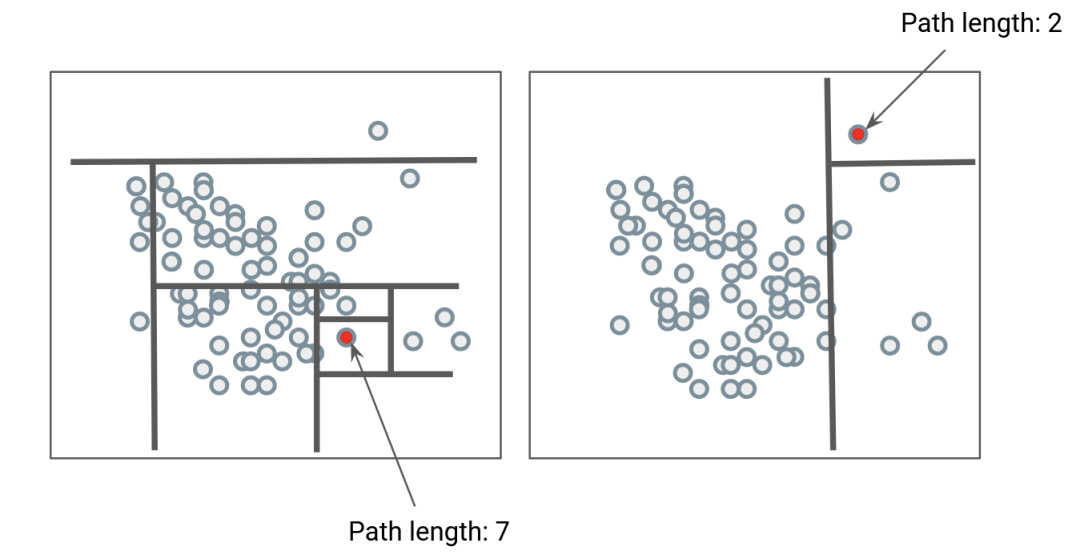
\includegraphics[width=10cm, scale=1]{images/iforest}
	\caption{I-Forest}
	\label{iforest}
\end{figure}
\subsubsection{INNE}
l rilevamento di anomalie basato sull'isolamento utilizzando ensemble di nearest-neighbour (INNE) \cite{bandaragoda2018isolation} è un metodo per rilevare anomalie in cui un ensemble di nearest-neighbor viene addestrato sui dati normali per identificare i punti di dati che sono isolati dal resto dei dati, che vengono considerati anomalie.

Il processo di solito funziona come segue:
\begin{enumerate}
\item Il set di dati viene diviso in un insieme di addestramento e di test.
\item L'ensemble di nearest-neighbor viene addestrato sull'insieme di addestramento utilizzando una tecnica come KNN o LOF.
\item L'ensemble di nearest-neighbor viene quindi utilizzato per identificare i punti di dati isolati nell'insieme di test. Questi punti di dati isolati vengono considerati anomalie.
\item Un punteggio di anomalia viene assegnato a ogni punto di dati, basato su quanto è isolato il punto dal resto dei dati. Più alto è il punteggio di anomalia, maggiore è la probabilità che il punto di dati sia un'anomalia.
\end{enumerate}

\subsubsection{Feature-Bagging}
Feature Bagging \cite{lazarevic2005feature} è un meta-estimator che adatta una serie di predittori di base a vari sotto-insiemi del dataset ed utilizza la media o altri metodi di combinazione per migliorare l'accuratezza predittiva e controllare l'over-fitting.
Le feature sono anch'esse campionate in modo casuale.
Per impostazione predefinita, viene utilizzato LOF come predittore di base. Tuttavia, è possibile utilizzare qualsiasi modello, come KNN e ABOD.
Il Feature Bagging costruisce innanzitutto \textit{n} sottoinsiemi selezionando casualmente un sottoinsieme di feature, il che induce la diversità dei predittori di base.
Infine, il punteggio di predizione viene generato facendo la media o prendendo il massimo.

\section{Modelli a rete neurale}
I metodi basati sulle reti neurali sono una sotto-categoria di metodi di Machine Learning che si basano su reti neurali.
Le reti neurali possono essere considerate come strutture che simulano il comportamento e il meccanismo del cervello umano. Come il cervello umano, l'unità di base della computazione è il neurone e questi sono collegati tra loro attraverso le sinapsi.  Il segnale propagato è proporzionale all'input ricevuto.
In primo luogo, c'è una serie di neuroni che si trovano all'ingresso della rete: questi sono chiamati neuroni di ingresso, che hanno il compito di raccogliere le informazioni da elaborare all'interno della rete.
Poi, c'è un neurone chiamato neurone di uscita, che ha il compito di restituire il risultato della computazione della rete. L'elaborazione avviene, in questo caso attraverso la somma ponderata degli ingressi. 
Ad ogni segnale di ingresso viene associato un peso, che è un punto fondamentale delle reti neurali, in quanto è attraverso questi pesi viene restituito un risultato piuttosto che un altro. Inoltre, al neurone di uscita è associato un ulteriore input chiamato bias: esso rappresenta la tendenza del neurone ad attivarsi o meno. Ovviamente, maggiore è il bias, maggiore è la tendenza del neurone ad attivarsi, poiché aggiunge più informazioni alla somma ponderata. Per semplificare i calcoli, il bias viene trattato come un neurone di ingresso aggiuntivo con segnale di ingresso sempre uguale a 1 e peso associato pari al bias scelto. A questo punto, il risultato della somma ponderata passa attraverso una funzione di attivazione, che restituisce il risultato effettivo.

Ci sono diversi tipi di reti neurali, tra cui:
\begin{itemize}
\item \textit{Reti feed-forward}: una semplice struttura di reti neurali in cui i dati scorrono in una direzione, dall'ingresso all'uscita.
\item \textit{Reti ricorrenti}: una struttura di reti neurali in cui i dati possono fluire in entrambe le direzioni, dall'ingresso all'uscita e viceversa.
\item  \textit{Reti convoluzionali}: una struttura di reti neurali utilizzata per lavorare con immagini e video, in cui vengono utilizzati filtri per estrarre caratteristiche dai dati di ingresso.
\item \textit{Reti autoencoder}: una struttura di reti neurali utilizzata per la riduzione della dimensionalità e l'apprendimento non supervisionato.
\item \textit{Reti generative}: una struttura di reti neurali utilizzata per generare nuovi dati, come ad esempio immagini, testo o suoni.
\end{itemize}


\subsection{Reti neurali profonde}
Le reti neurali vengono definite profonde quando hanno molti strati di neuroni. In generale, si considera una rete neurale profonda quando ha almeno tre strati nascosti, ovvero strati tra l'ingresso e l'uscita della rete. Un numero maggiore di strati consente alla rete di apprendere rappresentazioni più complesse dei dati.
\subsubsection{DeepSVDD}
\begin{figure}[t]
	\centering
	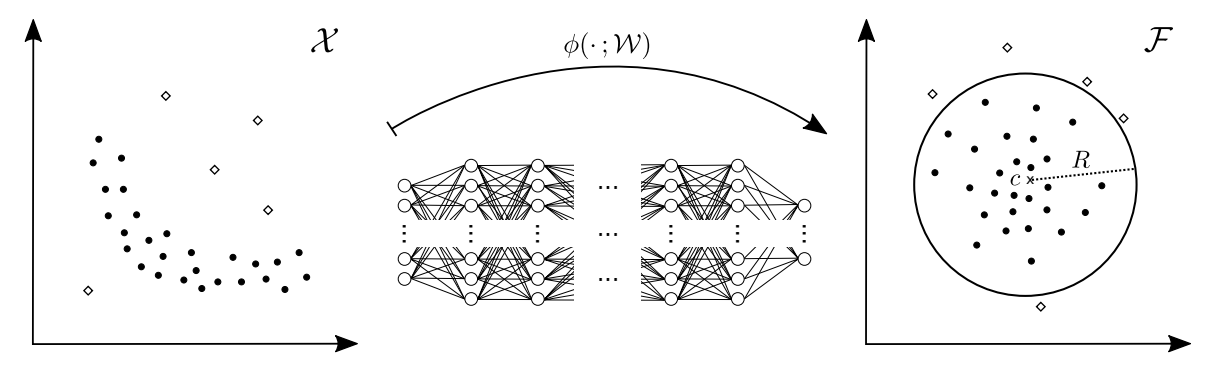
\includegraphics[width=10cm, scale=1]{images/deepsvdd}
	\caption{DeepSVDD}
	\label{deepsvdd}
\end{figure}

Deep Support Vector Data Description (DeepSVDD) \cite{ruff2018deepsvdd} è una rete neurale profonda che durante la fase di training punta a minimizzare il volume della ipersfera che racchiude la rappresentazione sui dati. Minimizzare il volume dell'ipersfera forza la rete neurale ad estrarre i fattori comuni di variazione dato che deve mappare i punti del dataset al centro della sfera.  La Figura \ref{deepsvdd} mostra le trasformazioni di DeepSVDD.

\subsection{Auto-Encoders}
Un Auto-Encoder (AE) \cite{aggarwal2015outlier} è una rete neurale che combina un encoder $E$ e un decoder $D$. L'encoder è un modulo che comprime i dati. Riceve come input il vettore di dati $W$ inerente ad un'osservazione del dataset e li mappa in un insieme di variabili latenti $Z$ che solitamente sono situati in uno spazio dimensionale minore. Il decoder è il secondo modulo il quale si occupa di decodificare le variabili latenti Z, rimappandole nello spazio originario di input come ricostruzione $\widehat{W}$. La differenza tra il vettore di dati $W$ e il vettore ricostruito $\widehat{W}$ è chiamata \textit{errore di ricostruzione}. Pertanto, l'obiettivo dell'addestramento mira a minimizzare questo errore. Nell'ambito dell'Anomaly Detection, viene utilizzato questo errore come score di anomalia: se un auto-encoder riesce a ricostruire senza errori un sample vuol dire che questo esprime caratteristiche normali; un sample anomalo invece porta l'auto-encoder a compiere errori nella fase di ricostruzione. L'architettura di un auto-encoder è presente nella Figura \ref{ae}.
\begin{figure}[t]
	\centering
	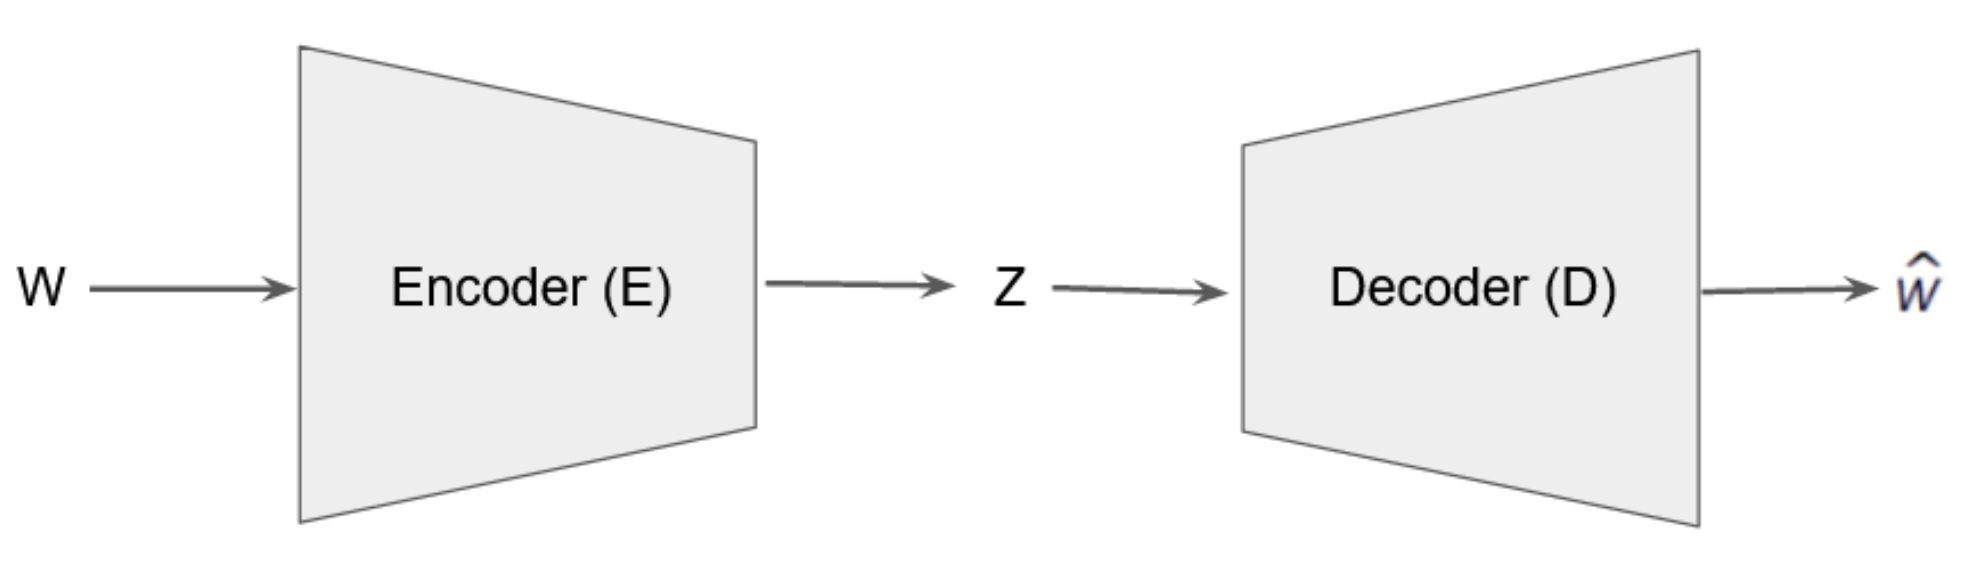
\includegraphics[width=10cm, scale=1]{images/ae}
	\caption{Auto-Encoder}
	\label{ae}
\end{figure}
\subsubsection{Variational-Autoencoders}
I Variational Autoencoders (VAE) \cite{kingma2013auto} ereditano parte dell'architettura dei classici AutoEncoders ma hanno profonde differenze. VAE è considerato un modello generativo e inoltre il suo encoder non solo produce una rappresentazione latente, ma anche una distribuzione di probabilità della rappresentazione latente $\mu$ e $\sigma$. Questo rende possibile generare nuovi sample semplicemente estraendo valori casuali dalla distribuzione di probabilità prodotta dall'encoder.
Il modello viene allenato per minimizzare la divergenza Kullback-Leibler (KL) tra la distribuzione di probabilità prodotta dall'encoder e una distribuzione nota (spesso una distribuzione normale) e allo stesso tempo massimizzare la capacità del decoder di ricostruire l'immagine originale (Figura \ref{vae}).
\begin{figure}[t]
	\centering
	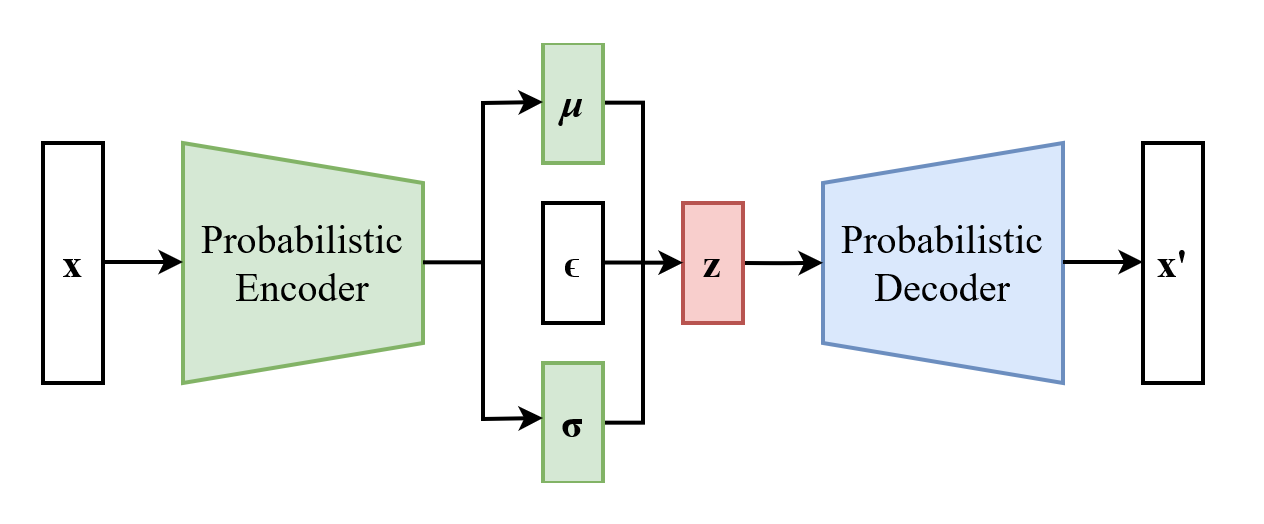
\includegraphics[width=10cm, scale=1]{images/vae}
	\caption{VAE}
	\label{vae}
\end{figure}

\subsection{LSTM}
Le LSTM (Long Short-Term Memory) sono un tipo di rete neurale artificiale utilizzata in problemi di elaborazione del linguaggio e predizione dei dati temporali. Sono state progettate per gestire problemi di "vanishing gradient" presenti in modelli di rete neurale tradizionali, consentendo una memorizzazione a lungo termine dei dati. Ciò significa che le LSTM possono tenere traccia di eventi che accadono molto tempo prima, il che è utile per comprendere il contesto.
Le reti LSTM sono composte da elementi detti \textit{unit} o \textit{celle} che a loro volta sono composte da dei \textit{gates}: uno di ingresso, uno di uscita e uno detto \textit{forget gate}. La cella ricorda i valori su intervalli di tempo arbitrari e i tre gate regolano il flusso di informazioni in entrata e in uscita. Le forget gate decidono quali informazioni scartare da uno stato precedente assegnando a quest'ultimo, rispetto all'ingresso corrente, un valore compreso tra 0 e 1. Un valore vicino a 1 significa mantenere l'informazione, mentre un valore di 0 significa scartarla. Le porte di ingresso decidono quali nuove informazioni memorizzare nello stato corrente, utilizzando lo stesso sistema delle forget gate. Le porte di uscita controllano quali informazioni dello stato corrente devono essere emesse, assegnando un valore da 0 a 1 alle informazioni, tenendo conto degli stati precedenti e di quello attuale. L'emissione selettiva di informazioni rilevanti dallo stato corrente consente alla rete LSTM di mantenere dipendenze utili a lungo termine per fare previsioni, sia nel tempo corrente che in quello futuro.

Le LSTM possono essere utilizzate per rilevare anomalie in dati temporali andando ad addestrare il modello sui dati "normali", per imparare una rappresentazione del comportamento normale dei dati. Quindi, quando nuovi dati vengono presentati al modello, possono essere utilizzati per generare una previsione e confrontare questa previsione con i dati effettivi. Se ci sono differenze significative tra la previsione e i dati effettivi, allora questi dati possono essere considerati anomali.


\subsection{Reti avversarie generative}
Le reti avversarie generative, o in breve GAN, sono un approccio alla modellazione generativa che utilizza metodi di apprendimento come le reti neurali convoluzionali.

La modellazione generativa è un task dell'apprendimento non supervisionato che prevede la scoperta e l'apprendimento automatico delle relazioni o delle variabili latenti all'interno dei dati di input in modo tale che il modello possa essere utilizzato per generare o produrre nuovi esempi che potrebbero essere stati plausibilmente ricavati dal set di dati originale.

Le GAN sono un modo di addestrare un modello generativo strutturando il problema in due parti: il modello generatore, che viene addestrato per generare nuovi esempi, e il modello discriminatore, che cerca di classificare gli esempi come reali (provenienti dal dominio) o falsi (generati). I due modelli vengono addestrati insieme in un gioco a somma zero (da qui adversarial), fino a quando il modello discriminatore viene ingannato circa la metà delle volte, il che significa che il modello generatore sta generando esempi plausibili. Lo schema della rete è presente in Figura \ref{gan}.
\begin{figure}[t]
	\centering
	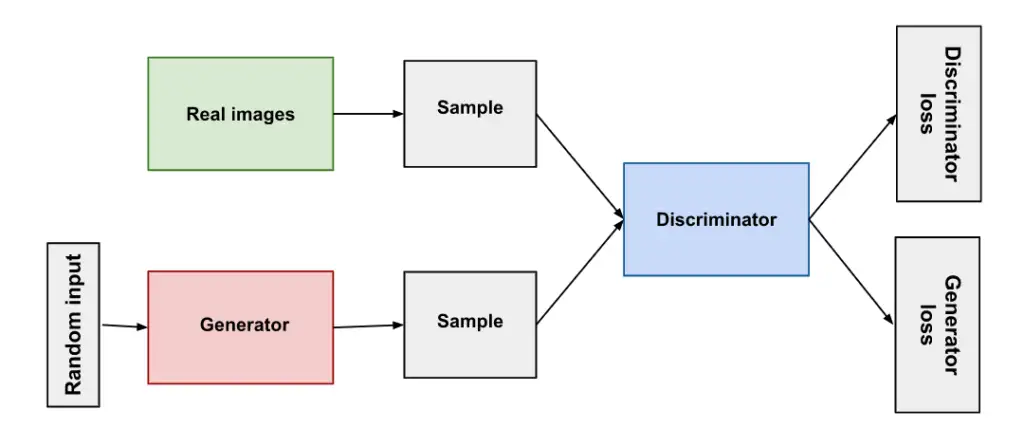
\includegraphics[width=12cm, scale=1]{images/gan}
	\caption{GAN}
	\label{gan}
\end{figure}

\subsubsection{AnoGAN}
AnoGAN (Anomaly GAN) \cite{schlegl2017unsupervised} è una tecnica di rilevamento di anomalie basata su GAN. Il modello AnoGAN utilizza un generatore GAN per generare una rappresentazione dei dati normali e quindi utilizza una rete neurale di rilevamento di anomalie per distinguere i dati normali dalle anomalie.

Il modello AnoGAN è composto da tre componenti principali:

\begin{enumerate}
\item Il generatore GAN che impara a generare dati che seguono la distribuzione dei dati normali.
\item Il discriminatore GAN che impara a distinguere i dati generati dai dati reali.
\item La rete neurale di rilevamento di anomalie che utilizza la rappresentazione generata dal generatore GAN per distinguere i dati normali dalle anomalie.
\end{enumerate}


\subsubsection{ALAD}
Adversarially Learned Anomaly Detection (ALAD) \cite{zenati2018adversarially} è una rete neurale che basa le sue fondamenta su AnoGAN. Ma a differenza di quest'ultima, include una GAN bi-direzionale e di conseguenza è presente un encoder al suo interno che mappa i dati di input in uno spazio latente ed utilizza l'errore di ricostruzione come score di anomalia.

\subsection{Reti neurali a grafo}
Le reti neurali basate su grafi (o GNN, Graph Neural Networks) sono una classe di modelli di apprendimento automatico che utilizzano strutture di dati a forma di grafo per rappresentare i dati. In questi modelli, i nodi del grafo rappresentano i sample e gli archi rappresentano le relazioni tra questi. Le GNN utilizzano un algoritmo di propagazione per aggiornare i valori dei nodi del grafo in base alle informazioni che si trovano sui nodi adiacenti.

\subsubsection{LUNAR}
LUNAR: Unifying Local Outlier Detection Methods via Graph Neural Networks \cite{goodge2022lunar} è un metodo per la rilevazione di anomalie che utilizza le reti neurali su grafi per apprendere la struttura locale dei dati. Il metodo si basa sull'idea che i punti di dati normali saranno simili ai loro punti di dati vicini, mentre i punti di dati anomali saranno dissimili.
Il processo di solito funziona come segue:
\begin{enumerate}
\item Viene costruito un grafo dai dati, dove ogni nodo rappresenta un punto di dati e gli archi vengono tracciati tra i punti di dati che vengono considerati simili.
\item Una rete neurale su grafi viene addestrata sul grafo per apprendere la struttura locale dei dati.
\item Dopo l'addestramento, la rete viene utilizzata per calcolare un punteggio di outlier per ogni punto di dati. Il punteggio di outlier rappresenta quanto dissimile è il punto di dati dai suoi punti di dati vicini.
\item I punti di dati con punteggi di outlier elevati vengono considerati anomalie.

\end{enumerate}

 È particolarmente utile per rilevare anomalie in dati che hanno una struttura complessa. Il metodo è in grado di modellare la struttura locale dei dati, il che lo rende efficace nel rilevare anomalie che potrebbero essere mancate da altri metodi.




\section{Thresholding}
Il problema del thresholding nella rilevazione di anomalie si riferisce alla sfida di determinare il valore di soglia appropriato che separi i punti di dati normali dai punti di dati anomali. Il valore di soglia viene solitamente utilizzato per assegnare un'etichetta di anomalia a ciascun punto di dati: i punti di dati con score di anomalia superiori alla soglia vengono considerati anomalie. Tuttavia, determinare il valore di soglia appropriato può essere difficile, poiché dipende dall'applicazione specifica e dall'insieme di dati.

Una delle principali sfide del thresholding è che solitamente si basa su una conoscenza a priori dei dati, che potrebbe non essere disponibile o potrebbe essere inaccurata. Inoltre, la distribuzione dei punti di dati e il numero di punti di dati anomali possono variare notevolmente tra diversi set di dati, rendendo difficile determinare un valore di soglia appropriato per tutti i set di dati.

Un'altra sfida del thresholding è che può essere difficile bilanciare il compromesso tra il numero di rilevamenti true-positive ed il numero di rilevamenti false-positive. Un valore di soglia troppo alto può causare molti falsi negativi, mentre un valore di soglia troppo basso può causare molti falsi positivi.
Sono proposti ora due metodi classici di thresholding ed un terzo metodo che verrà utilizzato nel Model Selection.

\subsection{IQR}
IQR \cite{https://doi.org/10.48550/arxiv.1509.02473} si basa sull'uso della deviazione interquartile (che è la differenza tra il terzo e il primo quartile) come base per determinare se un punto di dati è anomalo.

Il processo funziona come segue:
\begin{enumerate}
\item Viene calcolato il primo quartile (Q1), il terzo quartile (Q3) dei dati e la deviazione interquartile IQR dove $IQR = Q3-Q1$.
\item Viene definita la soglia inferiore come $Q1 - 1.5 \cdot IQR$ e la soglia superiore come $Q3 + 1.5 \cdot IQR$.
\item I punti di dati che si trovano al di fuori del range tra la soglia inferiore e la soglia superiore vengono considerati anomalie.
\end{enumerate}

Il vantaggio di questo metodo è che si basa solo sui dati e non richiede alcuna conoscenza a priori dei dati, quindi è un metodo semplice ed efficiente per determinare i valori di soglia. Tuttavia, questo metodo è sensibile ai valori estremi, quindi potrebbe non essere adatto per i dati con molti valori estremi.

\subsection{Z-Score}
Z-Score \cite{Bagdonavi_ius_2020} è una misura della distanza di un punto di dati dalla media dei dati in termini di deviazione standard. I punti di dati con Z-Score alti o troppo bassi vengono considerati anomalie.
Il processo funziona come segue:
\begin{enumerate}
\item Viene calcolata la media e la deviazione standard dei dati.
\item Viene calcolato lo Z-Score per ogni punto di dati utilizzando la formula $(x_i - avg) / std$.
\item Viene definita una soglia per i Z-Score, ad esempio 3 o -3 (che rappresentano rispettivamente 3 deviazioni standard sopra o sotto la media).
\item I punti di dati con Z-Score al di fuori della soglia vengono considerati anomalie.
\end{enumerate}
Anche questo metodo si basa solo sui dati e non richiede alcuna conoscenza a priori. Tuttavia, questo metodo presuppone che i dati seguano una distribuzione normale, quindi potrebbe non essere adatto per i dati non normalmente distribuiti. Inoltre, il valore della soglia deve essere scelto con attenzione in quanto può avere un impatto significativo sulle prestazioni del metodo.


\section{\texorpdfstring{$\gamma$}-GMM}
"ESTIMATING THE CONTAMINATION FACTOR’S DISTRIBUTION IN UNSUPERVISED ANOMALY DETECTION" \cite{https://doi.org/10.48550/arxiv.2210.10487} è un paper pubblicato da Lorenzo Perini et al.
Il problema trattato in questo paper consiste nella stima della distribuzione del fattore di contaminazione ($\gamma$) di un dataset non etichettato utilizzando un insieme di M rilevatori di anomalie non supervisionati. 
Per fattore di contaminazione si intende il valore, espresso in percentuale, della quantità di punti anomali in un dataset. 

Per affrontare questo problema, in questo paper viene proposto $\gamma$GMM, un approccio innovativo che utilizza un metodo bayesiano per stimare la distribuzione del fattore di contaminazione.
L'approccio $\gamma$GMM si compone di quattro fasi:
\begin{enumerate}
\item La prima fase consiste nella mappatura dei dati in uno spazio di anomalie a M dimensioni, dove le dimensioni corrispondono ai punteggi di anomalia assegnati dai M rilevatori di anomalie. In questo spazio, il pattern evidente è che "più alto è il punteggio, più anomalo è il dato".
\item La seconda fase consiste nel modellare i dati in questo spazio utilizzando un modello di miscela di Gaussiane con processo di Dirichlet (DPGMM). Si assume che ognuno dei tanti componenti di miscela contenga solo dati normali o solo dati anomali. Se si conoscesse quali componenti contengono anomalie, sarebbe possibile derivare facilmente la distribuzione posteriore di $\gamma$ come somma delle proporzioni di miscela dei componenti anomali. Tuttavia, in questo setting tale informazione non è disponibile.
\item La terza fase consiste nella stima della probabilità che i $k$ componenti più estremi siano anomalie. Ciò presenta tre sfide: (1) rappresentare ogni componente in uno spazio M-dimensionale utilizzando un unico valore per ordinarli dal più anomalo al meno anomalo, (2) calcolare la probabilità che il k-esimo componente sia anomalo dato che il (k-1)-esimo è tale, (3) derivare la probabilità obiettivo che esattamente $k$ componenti siano anomalie congiuntamente.
\item La quarta e ultima fase consiste nella stima della distribuzione posteriore del fattore di contaminazione ($\gamma$) utilizzando la probabilità congiunta e le proporzioni di miscela dei componenti.
Le quattro fasi di lavoro sono mostrate nella Figura \ref{ygmm1}.

\end{enumerate}
\begin{figure}[t]
	\centering
	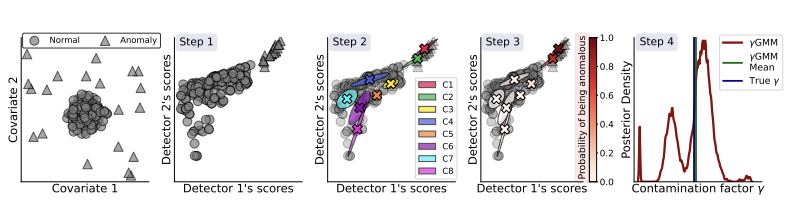
\includegraphics[width=14cm, scale=1]{images/ygmm1}
	\caption{I 4 step di $\gamma$GMM.}
	\label{ygmm1}
\end{figure}

In generale, l'approccio $\gamma$GMM fornisce una stima della distribuzione del fattore di contaminazione ($\gamma$) che può essere utilizzata per quantificare la probabilità che un dato campione sia anomalo rispetto a una distribuzione di dati normali. Inoltre, utilizzando un metodo bayesiano per la stima della distribuzione di $\gamma$, l'approccio $\gamma$GMM tiene conto delle incertezze nei parametri del modello. Ciò consente di ottenere una stima più precisa e robusta del fattore di contaminazione rispetto ai metodi tradizionali.
La formula utilizzata per la stima della distribuzione di $\gamma$ è la seguente:

\[p(\gamma | X) = \sum_{k=1}^{K} p(k | X) \sum_{i_1 < i_2 <...< i_k}^{m} p(\gamma | z_{i_1}, z_{i_2},..., z_{i_k}) p(z_{i_1}, z_{i_2},..., z_{i_k} | X)\]
dove $X$ è l'insieme di dati, $\gamma$ è il fattore di contaminazione, $k$ è il numero di componenti anomali, $z$ è il vettore di appartenenza ai componenti di miscela e $m$ è il numero di componenti di miscela.

All'interno del paper sono presenti anche i risultati degli esperimenti in cui il metodo $\gamma$GMM viene confrontato con numerosi metodi di thresholding tra cui IQR o Z-Score. I risultati sono incoraggianti e non solo ottiene il punteggio di MAE più basso (rispetto al true $\gamma$), ma la degradazione di una metrica supervisionata, come F-Measure, di un rilevatore di anomalie a cui è stato passato come fattore di contaminazione quanto generato dall'algoritmo di $\gamma$GMM, è la più bassa rispetto a tutti gli altri metodi di thresholding (Figura \ref{ygmm2}). 

\begin{figure}[t]
	\centering
	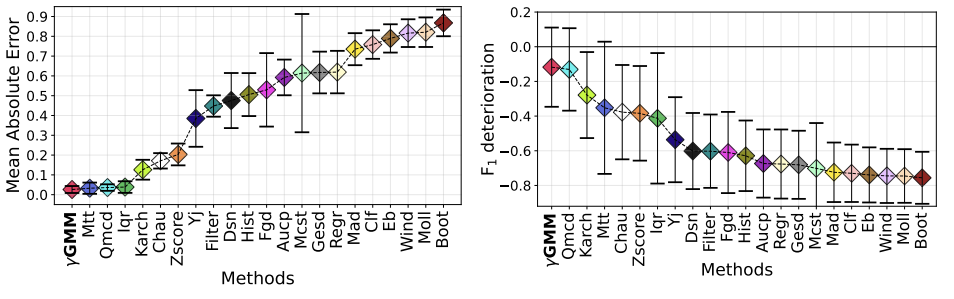
\includegraphics[width=14cm, scale=1]{images/ygmm2}
	\caption{Performance di $\gamma$GMM rispetto ad altre tecniche di thresholding. A sinistra i valori di MAE mentre a destra la F1-Deterioration.}
	\label{ygmm2}
\end{figure}

Per questo motivo, si è deciso di utilizzare questo metodo per la stima di contaminazione dei dati di SKF. Valore che poi è stato utilizzato come parametro ai modelli di Anomaly Detection utilizzato nel Model Selection.
